\chapter{Competencia imperfecta: el duopolio de Cournot}
\label{cap:duopolio}

\section{Entre el monopolio y la competencia}

Hasta acá la empresa decidía sola. Pero muchos mercados reales están dominados por \emph{pocas} empresas grandes (un \textbf{oligopolio}): telefonía, combustibles, supermercados. Ahí aparece algo nuevo y fascinante: el beneficio de cada empresa depende también de lo que haga la otra. Decidir se vuelve \textbf{estratégico} —hay que anticipar al rival—, y la herramienta para pensarlo es la \emph{teoría de juegos} \cite{gibbons}.

El modelo más clásico es el \textbf{duopolio de Cournot} (Augustin Cournot, 1838): dos empresas producen un bien homogéneo y compiten eligiendo \emph{cantidades} de forma simultánea. El precio de mercado surge de la cantidad total ofrecida.

\section{El problema de cada empresa}

Sean dos empresas con cantidades $q_1$ y $q_2$. La cantidad total es $Q = q_1 + q_2$ y el precio lo fija la demanda inversa del mercado, por ejemplo lineal:
\begin{equation}
p(Q) = a - b\,(q_1 + q_2).
\end{equation}
Si cada empresa tiene costo marginal constante $c$, el beneficio de la empresa 1 es
\begin{equation}
\Pi_1(q_1,q_2) = \big[a - b(q_1+q_2)\big]q_1 - c\,q_1 .
\end{equation}
Lo decisivo: $\Pi_1$ depende de $q_2$, que la empresa 1 \emph{no controla}. Lo que sí puede hacer es elegir su mejor $q_1$ \emph{para cada} valor posible de $q_2$.

\section{La función de mejor respuesta}

La empresa 1 maximiza su beneficio tomando $q_2$ como dado. Aplicando la CPO del Capítulo~\ref{cap:optimizacion} (derivar respecto de $q_1$ e igualar a cero):
\begin{equation}
\frac{\partial \Pi_1}{\partial q_1} = a - 2b\,q_1 - b\,q_2 - c = 0
\;\Longrightarrow\;
q_1 = \frac{a - c - b\,q_2}{2b}.
\label{eq:mejor_respuesta}
\end{equation}
Esta es la \textbf{función de mejor respuesta} (o reacción) de la empresa 1: su producción óptima \emph{en función} de lo que produzca la 2. Cuanto más produce la rival, menos le conviene producir a ella (las cantidades son «sustitutos estratégicos»). Por simetría, la empresa 2 tiene su propia mejor respuesta.

\section{El equilibrio de Nash-Cournot}

¿Dónde termina esta mutua anticipación? En el punto en que \textbf{ninguna empresa quiere cambiar su decisión dada la de la otra}: ambas están sobre su mejor respuesta a la vez. Eso es un \textbf{equilibrio de Nash} \cite{gibbons}. Por simetría $q_1^{*}=q_2^{*}=q^{*}$, y reemplazando en \eqref{eq:mejor_respuesta}:
\begin{equation}
q^{*} = \frac{a-c}{3b}, \qquad Q^{*} = 2q^{*} = \frac{2(a-c)}{3b}.
\end{equation}

\begin{ejemplo}[Un duopolio concreto]
Sea $p = 100 - (q_1+q_2)$ (es decir $a=100$, $b=1$) y costo marginal $c=10$. La mejor respuesta de la empresa 1 es $q_1 = (90 - q_2)/2$. En el equilibrio simétrico:
\[
q^{*} = \frac{100-10}{3} = 30, \qquad Q^{*} = 60, \qquad p^{*} = 100 - 60 = 40.
\]
El beneficio de cada empresa es $\Pi = (40-10)\cdot 30 = 900$.
\end{ejemplo}

\begin{figure}[htbp]
\centering
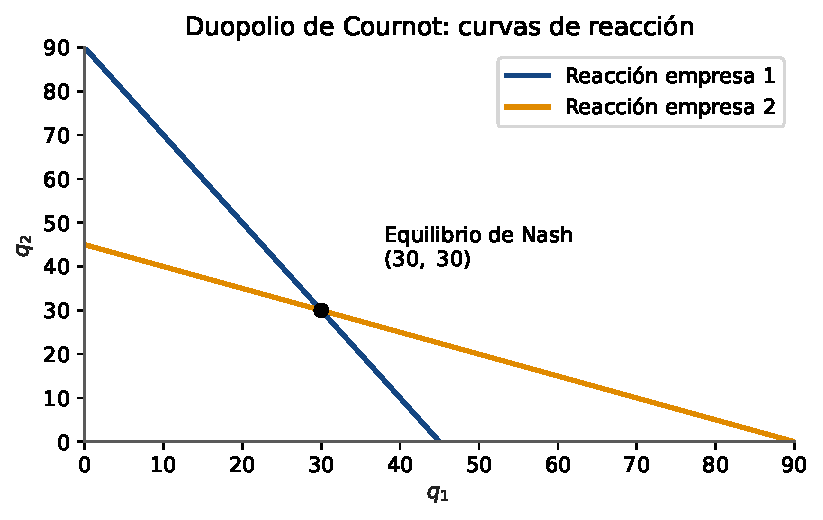
\includegraphics[width=0.72\linewidth]{figuras/cournot}
\caption{Las curvas de reacción de ambas empresas. Donde se cruzan, cada una está dando su mejor respuesta a la otra: ese punto es el equilibrio de Nash-Cournot.}
\label{fig:cournot}
\end{figure}

\section{Comparación: ¿cuánto importa la estructura del mercado?}

La gracia del modelo es comparar el duopolio con los dos extremos, usando los mismos números ($a=100$, $b=1$, $c=10$):

\begin{center}
\begin{tabular}{lccc}
\toprule
\textbf{Estructura} & \textbf{Cantidad total $Q$} & \textbf{Precio $p$} & \textbf{Beneficio total} \\
\midrule
Monopolio        & 45 & 55 & 2025 \\
Duopolio Cournot & 60 & 40 & 1800 \\
Competencia perfecta & 90 & 10 & 0 \\
\bottomrule
\end{tabular}
\end{center}

El patrón es nítido: a medida que aumenta la competencia (de 1 a 2 a muchas empresas), \textbf{la cantidad total sube, el precio baja y se acerca al costo marginal, y el beneficio extraordinario se disipa}. El consumidor gana con la competencia; las empresas la resisten. El duopolio queda, como era de esperar, a mitad de camino \cite{pindyck}. Con $n$ empresas idénticas, puede mostrarse que $Q = \tfrac{n}{n+1}\cdot\tfrac{a-c}{b}$, que tiende al resultado competitivo cuando $n\to\infty$.

\begin{ideabox}
\textbf{Por qué importa.} La teoría de juegos explica fenómenos que el modelo de empresa aislada no puede: guerras de precios, colusión, barreras de entrada, decisiones de capacidad. Es la base del análisis de la competencia y de la política antimonopolio (la «defensa de la competencia»).
\end{ideabox}

\begin{labbox}
En el laboratorio, el equilibrio de Cournot se resuelve planteando las dos funciones de mejor respuesta como un \emph{sistema de ecuaciones} y usando \texttt{sympy.solve} sobre $q_1$ y $q_2$ a la vez —es, otra vez, resolver un sistema, como en el Capítulo~\ref{cap:equilibrio}—. También puede graficarse el cruce de las dos curvas de reacción: el punto donde se cortan es el equilibrio de Nash. La teoría estratégica se vuelve, así, dos rectas que se intersecan en la pantalla.
\end{labbox}

\section{Síntesis del capítulo}

Cuando pocas empresas interactúan, decidir es anticipar. La función de mejor respuesta y el equilibrio de Nash resuelven el duopolio de Cournot, que se ubica entre el monopolio y la competencia perfecta. En el capítulo final pasamos del corto plazo de la producción al largo plazo de las decisiones de inversión.
